% ============================================================
% CAPITULO 21: REGLA DE LA CADENA, DERIVADA DIRECCIONAL Y GRADIENTE
% ============================================================

\chapter{Regla de la cadena, derivada direccional y gradientes} 

La regla de la cadena extiende formas de calcular las derivadas parciales de una función de acuerdo con varias técnicas ya estudiadas, las cuales se detallan a continuación

\section{Regla de la cadena}

\begin{theorem}[Regla de la cadena, Caso 1]
Si $z = f(x, y)$ es diferenciable y $x = g(t)$, $y = h(t)$ son funciones diferenciables de $t$, entonces $z$ es una función diferenciable de $t$ y
\[
\frac{dz}{dt} = \frac{\partial z}{\partial x}\frac{dx}{dt} + \frac{\partial z}{\partial y}\frac{dy}{dt}.
\]
\end{theorem}

\begin{pasos}[Protocolo para la regla de la cadena (Caso 1)] Para calcular la regla de la cadena en su primer caso se pueden seguir estos pasos: 

\begin{enumerate}
    \item \textbf{Identificar las dependencias}: Determinar cómo $z$ depende de $t$ a través de $x(t)$ e $y(t)$.
    \item \textbf{Calcular las derivadas parciales}: Calcular $\partial z/\partial x$ y $\partial z/\partial y$ en términos de $x$ e $y$.
    \item \textbf{Calcular las derivadas ordinarias}: Calcular $dx/dt$ y $dy/dt$.
    \item \textbf{Sustituir y sumar}: Sustituir $x(t)$ e $y(t)$ en las derivadas parciales y luego sustituir todos los términos en la fórmula de la regla de la cadena, sumando los productos.
\end{enumerate}
\end{pasos}

\begin{example}[Regla de la cadena, Caso 1]
Use la regla de la cadena para hallar $dz/dt$ para
\[
z = x^2 y - \sen y, \quad x = \sqrt{t^2 + 1}, \quad y = e^t.
\]
\begin{myproof}
Seguimos el protocolo para la regla de la cadena (Caso 1).
\begin{enumerate}
    \item \textbf{Identificar dependencias}: $z$ depende de $t$ a través de $x(t) = \sqrt{t^2+1}$ y $y(t) = e^t$.
    \item \textbf{Calcular derivadas parciales}:
    \[
    \frac{\partial z}{\partial x} = 2xy, \quad \frac{\partial z}{\partial y} = x^2 - \cos y.
    \]
    \item \textbf{Calcular derivadas ordinarias}:
    \[
    \frac{dx}{dt} = \frac{t}{\sqrt{t^2+1}}, \quad \frac{dy}{dt} = e^t.
    \]
    \item \textbf{Sustituir y sumar}:
    \[
    \frac{dz}{dt} = (2xy)\frac{dx}{dt} + (x^2 - \cos y)\frac{dy}{dt}.
    \]
    Sustituyendo $x$ e $y$:
    \[
    \frac{dz}{dt} = 2\left(\sqrt{t^2+1}\right)(e^t)\left(\frac{t}{\sqrt{t^2+1}}\right) + \left((t^2+1) - \cos(e^t)\right)(e^t).
    \]
    Simplificando:
    \[
    \frac{dz}{dt} = 2t e^t + \left(t^2 + 1 - \cos(e^t)\right)e^t = \boxed{\left(t^2 + 2t + 1 - \cos(e^t)\right)e^t}.
    \]
\end{enumerate}
\end{myproof}
\end{example}

\begin{prob}
El voltaje $V$ en un circuito eléctrico simple disminuye con lentitud a medida que la batería se gasta. La resistencia $R$ se incrementa lentamente cuando el resistor se calienta. Mediante la ley de Ohm, $V=IR$, determine cómo cambia la corriente $I$ en el momento en que $R=500\ \Omega$ , $I=0.06\  A$, $\frac{dV}{dt}=-0.02\ V/s$ y $\frac{dR}{dt}=0.04\ \Omega /s.$
\begin{myproof}
\textbf{Paso 1. Identificar la función y las tasas conocidas.}
$V=IR$. Datos: $R=500\,\Omega$, $I=0.06\,A$, $\dfrac{dV}{dt}=-0.02\,V/s$, $\dfrac{dR}{dt}=0.04\,\Omega/s$.

\textbf{Paso 2. Aplicar la regla de la cadena.}
\[
\frac{dV}{dt}=\frac{\partial V}{\partial I}\frac{dI}{dt}+\frac{\partial V}{\partial R}\frac{dR}{dt}
=R\frac{dI}{dt}+I\frac{dR}{dt}.
\]

\textbf{Paso 3. Sustituir y despejar $dI/dt$.}
\[
-0.02=500\,\frac{dI}{dt}+(0.06)(0.04)=500\,\frac{dI}{dt}+0.0024.
\]
\[
500\,\frac{dI}{dt}=-0.02-0.0024=-0.0224\implies
\frac{dI}{dt}=\frac{-0.0224}{500}=-0.0000448\ A/s.
\]

\textbf{Paso 4. Resultado.}
\[
\boxed{\frac{dI}{dt}\approx -4.48\times10^{-5}\ A/s}
\]
\end{myproof}
\end{prob}

\begin{prob}
El radio de un cono circular recto se incrementa a una razón de $5\ m/s$, mientras su altura disminuye a razón de $10\ m/s$. ¿A qué razón cambia el volumen del cono cuando el radio es $800\ m$ y la altura es de $200\ m$? Construya una representación de la situación.
\begin{myproof}
\textbf{Paso 1. Función de volumen y tasas conocidas.}
$V=\dfrac{\pi}{3}r^2h$. Datos: $r=800\,m$, $h=200\,m$, $\dfrac{dr}{dt}=5\,m/s$, $\dfrac{dh}{dt}=-10\,m/s$.

\textbf{Paso 2. Regla de la cadena.}
\[
\frac{dV}{dt}=\frac{\partial V}{\partial r}\frac{dr}{dt}+\frac{\partial V}{\partial h}\frac{dh}{dt}
=\frac{2\pi r h}{3}\cdot\frac{dr}{dt}+\frac{\pi r^2}{3}\cdot\frac{dh}{dt}.
\]

\textbf{Paso 3. Sustitución.}
\[
\frac{dV}{dt}
=\frac{2\pi(800)(200)}{3}(5)+\frac{\pi(800)^2}{3}(-10)
=\frac{1\,600\,000\,\pi}{3}-\frac{6\,400\,000\,\pi}{3}
=-\frac{4\,800\,000\,\pi}{3}\ m^3/s.
\]

\textbf{Paso 4. Resultado.}
\[
\boxed{\frac{dV}{dt}=-1\,600\,000\,\pi\ m^3/s\approx -5.03\times10^6\ m^3/s}
\]
\end{myproof}
\end{prob}

\begin{prob}
La longitud $l$, ancho $a$ y altura $h$ de una caja cambia con el tiempo. En un cierto instante, las dimensiones son $l= 5\ m,$ $a=3\ m$ y $h= 9\ m$, y se conoce que $a$ y $h$ se incrementan a razón de $0.3\ m/s$, en tanto que $l$ disminuye a razón de $0.5\ m/s.$ Encuentre en ese instante las razones a las cuales el área superficial de la caja cambia.
\begin{myproof}
\textbf{Paso 1. Función y tasas conocidas.}
$S=2la+2ah+2hl$. Datos: $l=5\,m$, $a=3\,m$, $h=9\,m$; $\dfrac{dl}{dt}=-0.5\,m/s$, $\dfrac{da}{dt}=\dfrac{dh}{dt}=0.3\,m/s$.

\textbf{Paso 2. Derivadas parciales de $S$.}
\[
\frac{\partial S}{\partial l}=2a+2h,\quad
\frac{\partial S}{\partial a}=2l+2h,\quad
\frac{\partial S}{\partial h}=2a+2l.
\]

\textbf{Paso 3. Regla de la cadena y sustitución.}
\[
\frac{dS}{dt}=(2a+2h)\frac{dl}{dt}+(2l+2h)\frac{da}{dt}+(2a+2l)\frac{dh}{dt}.
\]
\[
=(2(3)+2(9))(-0.5)+(2(5)+2(9))(0.3)+(2(3)+2(5))(0.3)
=24(-0.5)+28(0.3)+16(0.3)
=-12+8.4+4.8=1.2\ m^2/s.
\]

\textbf{Paso 4. Resultado.}
\[
\boxed{\frac{dS}{dt}=1.2\ m^2/s}
\]
\end{myproof}
\end{prob}

\begin{prob}
En un instante dado, la longitud de un cateto de un triángulo rectángulo es de $10\ cm$ y crece a tasa de $1\ cm/min,$ y la longitud del otro cateto es de $12\ cm.$ Calcule la tasa de variación de la medida del ángulo opuesto al cateto de 10 cm en ese instante.
\begin{myproof}
\textbf{Paso 1. Relación trigonométrica.}
Sea $\alpha$ el ángulo opuesto al cateto $a=10\,cm$ (con $\dfrac{da}{dt}=1\,cm/min$), y $b=12\,cm$ el otro cateto ($\dfrac{db}{dt}=0$). Entonces $\tan\alpha=\dfrac{a}{b}$.

\textbf{Paso 2. Diferenciación respecto a $t$.}
\[
\sec^2\!\alpha\;\frac{d\alpha}{dt}
=\frac{b\,\dfrac{da}{dt}-a\,\dfrac{db}{dt}}{b^2}
=\frac{\dfrac{da}{dt}}{b}.
\]

\textbf{Paso 3. Evaluación en el instante dado.}
\[
\tan\alpha=\frac{10}{12}=\frac{5}{6}\implies
\sec^2\!\alpha=1+\frac{25}{36}=\frac{61}{36}.
\]
\[
\frac{61}{36}\;\frac{d\alpha}{dt}=\frac{1}{12}\implies
\frac{d\alpha}{dt}=\frac{36}{12\cdot 61}=\frac{3}{61}\ \frac{\text{rad}}{\text{min}}.
\]

\textbf{Paso 4. Resultado.}
\[
\boxed{\dfrac{d\alpha}{dt}=\dfrac{3}{61}\ \text{rad/min}\approx 0.049\ \text{rad/min}}
\]
\end{myproof}
\end{prob}


Si hay dos variables independientes, usamos el segundo caso de la regla de la cadena: 
\begin{theorem}[Regla de la cadena, Caso 2]
Si $z = f(x, y)$ es diferenciable y $x = g(s, t)$, $y = h(s, t)$ son diferenciables, entonces $z$ es una función diferenciable de $s$ y $t$, y
\[
\frac{\partial z}{\partial s} = \frac{\partial z}{\partial x}\frac{\partial x}{\partial s} + \frac{\partial z}{\partial y}\frac{\partial y}{\partial s},
\]
\[
\frac{\partial z}{\partial t} = \frac{\partial z}{\partial x}\frac{\partial x}{\partial t} + \frac{\partial z}{\partial y}\frac{\partial y}{\partial t}.
\]
\end{theorem}

\begin{pasos}[Protocolo para la regla de la cadena (Caso 2)] El siguiente protocolo permite calcular la regla de la cadena cuando hay dos variables independientes:
\begin{enumerate}
    \item \textbf{Identificar las dependencias}: Determinar cómo $z$ depende de $s$ y $t$ a través de $x(s,t)$ e $y(s,t)$.
    \item \textbf{Calcular las derivadas parciales}: Calcular $\partial z/\partial x$ y $\partial z/\partial y$ en términos de $x$ e $y$.
    \item \textbf{Calcular las derivadas de las variables intermedias}: Calcular $\partial x/\partial s$, $\partial x/\partial t$, $\partial y/\partial s$, $\partial y/\partial t$.
    \item \textbf{Sustituir y sumar}: Sustituir y sumar para encontrar $\partial z/\partial s$ y $\partial z/\partial t$ siguiendo las fórmulas.
\end{enumerate}
\end{pasos}

\begin{example}[Regla de la cadena, Caso 2]
Si $z = \sen(xy)$, donde $x = s^2 + t$ e $y = \ln(s t)$, calcule $\partial z/\partial s$ y $\partial z/\partial t$.
\begin{myproof}
Seguimos el protocolo para la regla de la cadena (Caso 2).
\begin{enumerate}
    \item \textbf{Identificar dependencias}: $z$ depende de $s$ y $t$ a través de $x(s,t) = s^2 + t$ e $y(s,t) = \ln(st)$.
    \item \textbf{Calcular derivadas parciales de $z$}:
    \[
    \frac{\partial z}{\partial x} = y \cos(xy), \quad \frac{\partial z}{\partial y} = x \cos(xy).
    \]
    \item \textbf{Calcular derivadas de $x$ e $y$}:
    \[
    \frac{\partial x}{\partial s} = 2s, \quad \frac{\partial x}{\partial t} = 1,
    \]
    \[
    \frac{\partial y}{\partial s} = \frac{1}{s}, \quad \frac{\partial y}{\partial t} = \frac{1}{t}.
    \]
    \item \textbf{Sustituir y sumar}:
    \[
    \frac{\partial z}{\partial s} = (y \cos(xy))(2s) + (x \cos(xy))\left(\frac{1}{s}\right)
    \]
    \[
    \frac{\partial z}{\partial t} = (y \cos(xy))(1) + (x \cos(xy))\left(\frac{1}{t}\right).
    \]
    Sustituyendo $x$ e $y$:
    \[
    \frac{\partial z}{\partial s} = \boxed{\cos((s^2+t)\ln(st))\left(2s \ln(st) + \frac{s^2+t}{s}\right)},
    \]
    \[
    \frac{\partial z}{\partial t} = \boxed{\cos((s^2+t)\ln(st))\left(\ln(st) + \frac{s^2+t}{t}\right)}.
    \]
\end{enumerate}
\end{myproof}
\end{example}



\section{Derivación implícita}

Cuando una función $z = f(x, y)$ no se da explícitamente, sino que está definida implícitamente por una ecuación $F(x, y, z) = 0$, podemos hallar sus derivadas parciales utilizando la regla de la cadena.

\begin{theorem}[Derivación implícita para funciones de varias variables]
Si una ecuación $F(x, y, z) = 0$ define implícitamente a $z$ como una función diferenciable de $x$ e $y$, entonces
\[
\frac{\partial z}{\partial x} = -\frac{F_x}{F_z}, \quad \frac{\partial z}{\partial y} = -\frac{F_y}{F_z}, \quad \text{siempre que } F_z \neq 0.
\]
\end{theorem}

\begin{rem}[Caso de una ecuación $F(x,y)=0$]
Si una ecuación $F(x,y)=0$ define implícitamente $y=y(x)$, el mismo argumento
(regla de la cadena aplicada a $F(x,y(x))=0$) da
\[
  \frac{dy}{dx}=-\frac{F_x}{F_y},\qquad F_y\neq 0.
\]
\end{rem}

\begin{prob}
Halle $\dfrac{dy}{dx}$ si $\cos(x+y)=y\,\sen x$.
\begin{myproof}
\textbf{Paso 1. Definir $F$.}
$F(x,y)=\cos(x+y)-y\,\sen x=0$.

\textbf{Paso 2. Parciales.}
\[
  F_x=-\sen(x+y)-y\cos x,\qquad
  F_y=-\sen(x+y)-\sen x.
\]

\textbf{Paso 3. Aplicar la fórmula.}
\[
  \frac{dy}{dx}=-\frac{F_x}{F_y}
  =-\frac{-\sen(x+y)-y\cos x}{-\sen(x+y)-\sen x}.
\]

\textbf{Paso 4. Simplificar.}
\[
  \boxed{\ \frac{dy}{dx}=-\frac{\sen(x+y)+y\cos x}{\sen(x+y)+\sen x}.\ }
\]
\end{myproof}
\end{prob}

\begin{pasos}[Protocolo para derivación implícita de $z$ definida por $F(x, y, z) = 0$] Es posible aplicar el siguiente protocolo para calcular la derivada implícita en varias variables:
\begin{enumerate}
    \item \textbf{Definir la función $F$}: Reordenar la ecuación para que un lado sea $0$ y definir $F(x, y, z)$ como el otro lado.
    \item \textbf{Calcular las derivadas parciales de $F$}: Calcular $F_x$, $F_y$ y $F_z$.
    \item \textbf{Aplicar las fórmulas}: Sustituir las derivadas en las fórmulas $\partial z/\partial x = -F_x/F_z$ y $\partial z/\partial y = -F_y/F_z$.
    \item \textbf{Simplificar (opcional)}: Simplificar la expresión resultante.
\end{enumerate}
\end{pasos}

\begin{example}[Derivación implícita]
Dada la ecuación $3yz^2 - e^{4x}\cos(4z) - 3y^2 = 4$, calcule $\partial z/\partial x$ y $\partial z/\partial y$.
\begin{myproof}
Seguimos el protocolo para derivación implícita.
\begin{enumerate}
    \item \textbf{Definir $F$}:
    \[
    F(x, y, z) = 3yz^2 - e^{4x}\cos(4z) - 3y^2 - 4.
    \]
    \item \textbf{Calcular las derivadas parciales de $F$}:
    \[
    F_x = -4e^{4x}\cos(4z),
    \]
    \[
    F_y = 3z^2 - 6y,
    \]
    \[
    F_z = 6yz + 4e^{4x}\sen(4z).
    \]
    \item \textbf{Aplicar las fórmulas}:
    \[
    \frac{\partial z}{\partial x} = -\frac{F_x}{F_z} = -\frac{-4e^{4x}\cos(4z)}{6yz + 4e^{4x}\sen(4z)} = \frac{4e^{4x}\cos(4z)}{6yz + 4e^{4x}\sen(4z)},
    \]
    \[
    \frac{\partial z}{\partial y} = -\frac{F_y}{F_z} = -\frac{3z^2 - 6y}{6yz + 4e^{4x}\sen(4z)} = \frac{6y - 3z^2}{6yz + 4e^{4x}\sen(4z)}.
    \]
    \item \textbf{Simplificar y concluir}:
    \[
    \boxed{\frac{\partial z}{\partial x} = \frac{4e^{4x}\cos(4z)}{6yz + 4e^{4x}\sen(4z)}},\qquad
    \boxed{\frac{\partial z}{\partial y} = \frac{6y - 3z^2}{6yz + 4e^{4x}\sen(4z)}}.
    \]
\end{enumerate}
\end{myproof}
\end{example}

\begin{prob}
Si $z = e^{xy}$, $x = s t$, $y = s + t$, encuentre $\partial z/\partial s$ y $\partial z/\partial t$.
\begin{myproof}
\textbf{Paso 1. Derivadas parciales de $z$ respecto a $x$ e $y$.}
\[
\frac{\partial z}{\partial x} = y e^{xy},\qquad \frac{\partial z}{\partial y} = x e^{xy}.
\]

\textbf{Paso 2. Derivadas de $x$ e $y$ respecto a $s$ y $t$.}
\[
\frac{\partial x}{\partial s}=t,\quad \frac{\partial x}{\partial t}=s,\quad
\frac{\partial y}{\partial s}=1,\quad \frac{\partial y}{\partial t}=1.
\]

\textbf{Paso 3. Regla de la cadena (Caso 2).}
\[
\frac{\partial z}{\partial s}
= ye^{xy}\cdot t + xe^{xy}\cdot 1
= (yt+x)e^{xy}.
\]
Sustituyendo $x=st$, $y=s+t$:
\[
yt+x = (s+t)t+st = st+t^2+st = t^2+2st = t(t+2s).
\]
\[
\frac{\partial z}{\partial t}
= ye^{xy}\cdot s + xe^{xy}\cdot 1
= (ys+x)e^{xy}.
\]
Sustituyendo:
\[
ys+x = (s+t)s+st = s^2+st+st = s^2+2st = s(s+2t).
\]

\textbf{Paso 4. Resultado.}
\[
\boxed{\frac{\partial z}{\partial s} = t(t+2s)\,e^{st(s+t)},\qquad
\frac{\partial z}{\partial t} = s(s+2t)\,e^{st(s+t)}}
\]
\end{myproof}
\end{prob}

\begin{rem}[Derivadas de segundo orden por la cadena]
Al derivar por segunda vez, cada parcial $f_x$ y $f_y$ \emph{sigue siendo}
función de las variables intermedias, de modo que se le vuelve a aplicar la
regla de la cadena. Conviene tratar $f_x$ y $f_y$ como nuevas funciones y
derivarlas igual que a $f$.
\end{rem}

\begin{prob}[Segunda derivada en coordenadas polares]
Sea $w=f(x,y)$ con $x=r\cos\theta$, $y=r\,\sen\theta$. Exprese
$\dfrac{\partial^2 w}{\partial r^2}$ en términos de las parciales de $f$.
\begin{myproof}
\textbf{Paso 1. Primera derivada $w_r$.}
Como $x_r=\cos\theta$ y $y_r=\sen\theta$,
\[
  w_r=f_x\,x_r+f_y\,y_r=f_x\cos\theta+f_y\,\sen\theta.
\]

\textbf{Paso 2. Derivar de nuevo respecto a $r$.}
Al derivar respecto a $r$, $\theta$ es constante y $f_x$, $f_y$ son funciones
de $(x,y)$; reaplicando la cadena:
\[
  \frac{\partial}{\partial r}(f_x)=f_{xx}\cos\theta+f_{xy}\,\sen\theta,\qquad
  \frac{\partial}{\partial r}(f_y)=f_{yx}\cos\theta+f_{yy}\,\sen\theta.
\]

\textbf{Paso 3. Combinar.}
\[
  w_{rr}=\cos\theta\,\frac{\partial}{\partial r}(f_x)
        +\sen\theta\,\frac{\partial}{\partial r}(f_y).
\]

\textbf{Paso 4. Resultado.}
Usando $f_{xy}=f_{yx}$,
\[
  \boxed{\ \frac{\partial^2 w}{\partial r^2}
  =f_{xx}\cos^2\theta+2f_{xy}\cos\theta\,\sen\theta+f_{yy}\,\sen^2\theta.\ }
\]
\end{myproof}
\end{prob}

\begin{prob}
La presión de un gas ideal es $P=\dfrac{kT}{V}$, con $k$ constante. En cierto
proceso la temperatura y el volumen varían con el tiempo según $T(t)=T_0+at$ y
$V(t)=V_0+bt$. Halle $\dfrac{dP}{dt}$ y $\dfrac{d^2P}{dt^2}$ en términos de
$t$ (use la regla de la cadena y la derivada de un cociente).
\end{prob}





\begin{prob}
Calcule $\partial z/\partial x$ y $\partial z/\partial y$ para la función $z$ definida implícitamente por $x^2 y - y^2 z + z^3 = 1$.
\begin{myproof}
Definimos $F(x,y,z)=x^2y-y^2z+z^3-1$.

\textbf{Paso 1. Derivadas parciales de $F$.}
\[
F_x = 2xy,\qquad F_y = x^2-2yz,\qquad F_z = -y^2+3z^2.
\]

\textbf{Paso 2. Aplicar la fórmula de derivación implícita.}
\[
\frac{\partial z}{\partial x} = -\frac{F_x}{F_z}
= -\frac{2xy}{3z^2-y^2},\qquad
\frac{\partial z}{\partial y} = -\frac{F_y}{F_z}
= -\frac{x^2-2yz}{3z^2-y^2}.
\]

\textbf{Paso 3. Verificación de hipótesis.}
La fórmula es válida siempre que $F_z=3z^2-y^2\neq 0$.

\textbf{Paso 4. Resultado.}
\[
\boxed{\frac{\partial z}{\partial x}=-\frac{2xy}{3z^2-y^2},\qquad
\frac{\partial z}{\partial y}=-\frac{x^2-2yz}{3z^2-y^2}}
\qquad(3z^2\neq y^2)
\]
\end{myproof}
\end{prob}

\section{Gradiente}
%%==========================================================

Recordemos que las derivadas parciales de una función $f(x,y)$,
denotadas $f_x(x,y)$ y $f_y(x,y)$, indican cómo cambia la función
cuando nos movemos a lo largo de los ejes $x$ e $y$, respectivamente.
Es decir, muestran la pendiente de la recta tangente a la superficie
$z=f(x,y)$ en esas direcciones específicas. El objetivo de esta sección
es extender esta idea y aprender a medir cómo cambia la función en
\emph{cualquier} dirección, no solo a lo largo de los ejes. Esta medida
se llama \textbf{derivada direccional}. Antes de definirla,
necesitamos conocer un concepto clave: el \textbf{vector gradiente}.

\begin{definition}[Gradiente de una función escalar]
Sea $f$ una función escalar de dos o tres variables.
\begin{itemize}
    \item Si $f(x,y)$ es una función de dos variables, el \textbf{gradiente}
    de $f$ es el campo vectorial $\nabla f$ definido por:
    \[
    \nabla f(x,y) = \langle f_x(x,y),\, f_y(x,y) \rangle
                  = \frac{\partial f}{\partial x}\,\mathbf{i}
                    + \frac{\partial f}{\partial y}\,\mathbf{j}.
    \]
    \item Si $f(x,y,z)$ es una función de tres variables, su gradiente es:
    \[
    \nabla f(x,y,z) = \langle f_x(x,y,z),\, f_y(x,y,z),\,
    f_z(x,y,z) \rangle
    = \frac{\partial f}{\partial x}\,\mathbf{i}
      + \frac{\partial f}{\partial y}\,\mathbf{j}
      + \frac{\partial f}{\partial z}\,\mathbf{k}.
    \]
\end{itemize}
\end{definition}

\begin{rem}
El símbolo $\nabla$ se lee \emph{nabla} o \emph{del}. El gradiente
transforma una función escalar en un campo vectorial: en cada punto del
dominio, asigna un vector cuyas componentes son las derivadas parciales
de $f$. Este vector contiene toda la información de primer orden sobre
el comportamiento de $f$ en ese punto.
\end{rem}

\begin{example}[Cálculo del gradiente]
Encuentre el gradiente de $f(x,y) = x^2 \sen y + e^{xy}$.
\begin{myproof}
\textbf{Paso 1. Derivada parcial $f_x$.}
\[
f_x(x,y) = 2x \sen y + y e^{xy}.
\]

\textbf{Paso 2. Derivada parcial $f_y$.}
\[
f_y(x,y) = x^2 \cos y + x e^{xy}.
\]

\textbf{Paso 3. Ensamblaje del gradiente.}
\[
\nabla f(x,y) = \langle f_x, f_y\rangle = (2x \sen y + y e^{xy})\,\mathbf{i}+(x^2 \cos y + x e^{xy})\,\mathbf{j}.
\]

\textbf{Paso 4. Resultado.}
\[
\boxed{\nabla f(x,y) = (2x \sen y + y e^{xy})\,\mathbf{i}
              + (x^2 \cos y + x e^{xy})\,\mathbf{j}}
\]
\end{myproof}
\end{example}

El operador gradiente satisface propiedades algebraicas que lo convierten
en una herramienta flexible. Estas propiedades se deducen directamente de
la linealidad de la derivación parcial y de las reglas del producto y
cociente para funciones escalares.

\begin{theorem}[Propiedades del gradiente]
Sean $f$ y $g$ funciones escalares diferenciables de dos o tres
variables, y sea $k\in\mathbb{R}$ una constante. Entonces:
\begin{enumerate}
    \item \textbf{Linealidad:}
    $\nabla(f \pm g) = \nabla f \pm \nabla g$.
    \item \textbf{Multiplicación por constante:}
    $\nabla(kf) = k\,\nabla f$.
    \item \textbf{Regla del producto:}
    $\nabla(fg) = f\,\nabla g + g\,\nabla f$.
    \item \textbf{Regla del cociente:}
    $\nabla\left(\dfrac{f}{g}\right) =
    \dfrac{g\,\nabla f - f\,\nabla g}{g^2}$, siempre que $g\neq 0$.
\end{enumerate}
\end{theorem}


Por otro lado, el gradiente tiene una interpretación geométrica interesante:



El vector gradiente $\nabla f(x_0,y_0)$ en un punto posee tres
propiedades geométricas fundamentales que lo convierten en el objeto
central del análisis local de funciones de varias variables.

\begin{enumerate}
    \item \textbf{Dirección de mayor aumento:} $\nabla f(x_0,y_0)$
    apunta en la dirección en la que la función $f$ crece más
    rápidamente desde el punto $(x_0,y_0)$.
    \item \textbf{Magnitud:} La longitud del vector gradiente,
    $||\nabla f(x_0,y_0)||$, es la tasa máxima de cambio de $f$ en ese
    punto.
    \item \textbf{Perpendicularidad:} $\nabla f(x_0,y_0)$ es ortogonal
    (perpendicular) a las curvas de nivel de $f$, es decir, a las curvas
    donde $f(x,y) = k$ para alguna constante $k$.
\end{enumerate}

\begin{figure}[H]
\centering
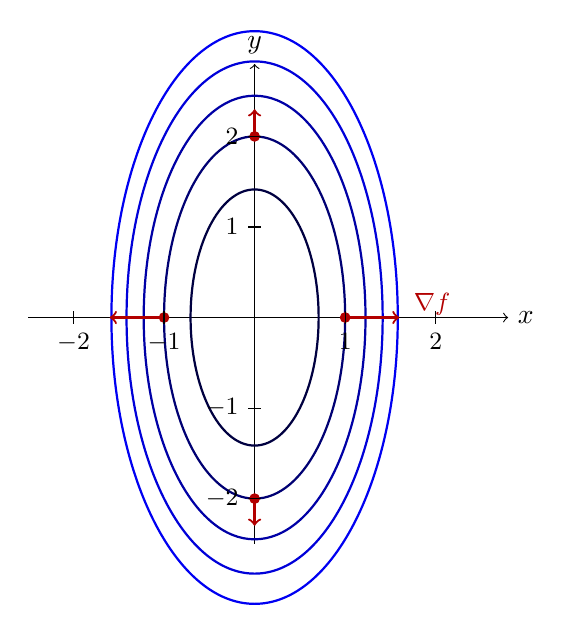
\begin{tikzpicture}[scale=1.15]
    \draw[thin,->] (-2.5,0) -- (2.8,0) node[right] {$x$};
    \draw[thin,->] (0,-2.5) -- (0,2.8) node[above] {$y$};
    % Curvas de nivel de f(x,y)=x²+y²/4 (elipses: x²+y²/4=c)
    % Semiejes: a=√c, b=2√c
    \foreach \c/\col in {0.5/blue!25!black, 1/blue!45!black, 1.5/blue!65!black, 2/blue!85!black, 2.5/blue!95!black}{
        \pgfmathsetmacro{\a}{sqrt(\c)}
        \pgfmathsetmacro{\b}{2*sqrt(\c)}
        \draw[thick, \col] (0,0) ellipse ({\a} and {\b});
    }
    % Vectores gradiente ∇f=(2x, y/2) en 4 puntos
    % Escala ×0.3 para que quepan en la figura
    % Punto 1: (1, 0) → ∇f=(2,0), escalado→(0.6,0)
    \draw[->, thick, red!70!black] (1,0) -- (1.6,0);
    % Punto 2: (0, 2) → ∇f=(0,1), escalado→(0,0.3)
    \draw[->, thick, red!70!black] (0,2) -- (0,2.3);
    % Punto 3: (-1,0) → ∇f=(-2,0), escalado→(-0.6,0)
    \draw[->, thick, red!70!black] (-1,0) -- (-1.6,0);
    % Punto 4: (0,-2) → ∇f=(0,-1), escalado→(0,-0.3)
    \draw[->, thick, red!70!black] (0,-2) -- (0,-2.3);
    % Puntos base
    \foreach \px/\py in {1/0, 0/2, -1/0, 0/-2}
        \filldraw[red!70!black] (\px,\py) circle (1.5pt);
    % Etiqueta gradiente
    \node[anchor=west, red!70!black] at (1.65,0.15) {\small $\nabla f$};
    % Marcas de eje
    \foreach \x in {-2,-1,1,2}
        \draw[thin] (\x,0.07)--(\x,-0.07) node[below] {\small $\x$};
    \foreach \y in {-2,-1,1,2}
        \draw[thin] (0.07,\y)--(-0.07,\y) node[left] {\small $\y$};
\end{tikzpicture}
\caption{Curvas de nivel de $f(x,y)=x^2+\tfrac{y^2}{4}$ (elipses)
         con vectores $\nabla f$ en cuatro puntos, perpendiculares
         a las curvas de nivel}
\label{fig:gradiente_curvas_nivel}
\end{figure}

\begin{rem}
La propiedad de perpendicularidad merece atención: si una curva de nivel
está parametrizada por $\mathbf{r}(t) = (x(t), y(t))$ con
$f(\mathbf{r}(t)) = k$, entonces derivando respecto a $t$ se obtiene
$\nabla f(\mathbf{r}(t))\cdot \mathbf{r}'(t) = 0$, lo que prueba que el
gradiente es normal a la curva de nivel en cada punto. Esta observación
será clave más adelante para construir planos tangentes a superficies
dadas en forma implícita.
\end{rem}

%%----------------------------------------------------------
\section{Derivada direccional}
%%----------------------------------------------------------

Con el gradiente como herramienta auxiliar, se puede ahora definir la derivada direccional. Intuitivamente, la derivada direccional mide la tasa de cambio de $f$ cuando nos movemos desde un punto dado en una dirección específica, representada por un vector unitario.

\begin{definition}[Derivada direccional]
La \textbf{derivada direccional} de $f(x,y)$ en el punto
$(x_0,y_0)$ y en la dirección del vector unitario
$\mathbf{u} = \langle u_1, u_2 \rangle$ está dada por:
\[
D_{\mathbf{u}} f(x_0,y_0)
= \lim_{h \to 0} \frac{f(x_0 + h u_1,\, y_0 + h u_2) - f(x_0,y_0)}{h},
\]
siempre que el límite exista.
\end{definition}

\begin{rem}
La derivada direccional generaliza las derivadas parciales: si
$\mathbf{u} = \mathbf{i} = \langle 1,0 \rangle$, entonces
$D_{\mathbf{i}} f = f_x$; si $\mathbf{u} = \mathbf{j} = \langle 0,1
\rangle$, entonces $D_{\mathbf{j}} f = f_y$. La exigencia de que
$\mathbf{u}$ sea unitario es crucial: si no lo fuera, el cociente
incremental no mediría tasa de cambio por unidad de longitud recorrida.
\end{rem}

Geométricamente, el vector $\mathbf{u}$ determina una recta $L$ que
contiene al punto $(x_0,y_0)$. El plano que contiene a $L$ y es
perpendicular al plano $xy$ corta a la superficie $z=f(x,y)$ en una
curva $C$. La recta tangente a la curva $C$ en el punto
$(x_0,y_0,f(x_0,y_0))$ tiene como pendiente la derivada direccional
$D_{\mathbf{u}} f(x_0,y_0)$.

El siguiente teorema proporciona la fórmula práctica para calcular la
derivada direccional sin recurrir al límite.

\begin{figure}[H]
\centering
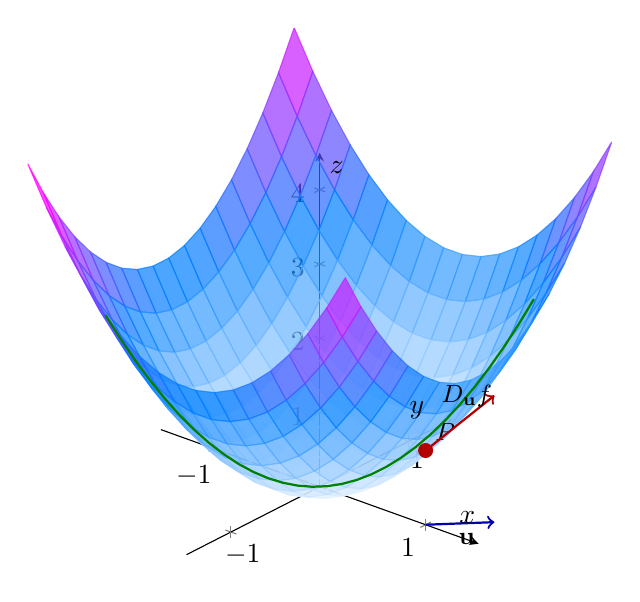
\begin{tikzpicture}
\begin{axis}[
    view={40}{28},
    xlabel={$x$}, ylabel={$y$}, zlabel={$z$},
    axis lines=center,
    tick style={thin},
    zmin=0, zmax=4.5,
    xtick={-1,1}, ytick={-1,1}, ztick={1,2,3,4},
    width=9cm, height=9cm,
]
    % Superficie z = x² + y²
    \addplot3[
        surf, shader=flat corner,
        samples=18, domain=-1.5:1.5,
        opacity=0.70, colormap/cool,
    ] {x^2 + y^2};
    % Punto P = (1, 0, 1)
    \addplot3[only marks, mark=*, mark size=2.5pt, red!70!black]
        coordinates {(1,0,1)};
    \node[above right] at (axis cs:1,0,1) {\small $P$};
    % Dirección u = (cos45°, sin45°) ≈ (0.707, 0.707) en plano xy
    % Plano vertical x=y: corta z=x²+y² en z=2x² (param: x=t, y=t, z=2t²)
    \addplot3[
        thick, green!50!black,
        domain=-1.1:1.1, samples=30, samples y=0,
    ] ({x},{x},{2*x^2});
    % Recta tangente en P=(1,0,1): pendiente D_u f = ∇f·u = (2,0)·(0.707,0.707)=√2
    % z - 1 = √2*(t - 0) donde t mide arco desde P en dirección u
    % Parametrizado: (1+0.707s, 0.707s, 1+1.414s)
    \draw[->, thick, red!70!black]
        (axis cs:1,0,1) -- (axis cs:{1+0.707*0.5},{0.707*0.5},{1+1.414*0.5});
    \node[above] at (axis cs:{1+0.707*0.3},{0.707*0.3},{1+1.414*0.3})
        {\small $D_{\mathbf{u}}f$};
    % Vector u en plano xy
    \draw[->, thick, blue!70!black]
        (axis cs:1,0,0) -- (axis cs:{1+0.707*0.5},{0.707*0.5},0);
    \node[below] at (axis cs:{1+0.707*0.3},{0.707*0.3},0)
        {\small $\mathbf{u}$};
\end{axis}
\end{tikzpicture}
\caption{Derivada direccional $D_{\mathbf{u}}f(P)$ como pendiente de la curva
         de intersección de la superficie $z=f(x,y)$ con el plano vertical
         en dirección $\mathbf{u}$}
\label{fig:derivada_direccional}
\end{figure}

\begin{theorem}[Fórmula del gradiente para la derivada direccional]
Sea $f$ una función diferenciable en el punto $p=(a,b)$, y sea
$\mathbf{u}=\langle u_1,u_2\rangle$ un vector unitario. Entonces:
\[
D_{\mathbf{u}} f(p) = \nabla f(p) \cdot \mathbf{u}
= f_x(a,b) u_1 + f_y(a,b) u_2.
\]
Si el vector unitario forma un ángulo $\theta$ con el eje $x$ positivo,
entonces $\mathbf{u} = \langle \cos\theta, \sen\theta \rangle$ y la
fórmula se convierte en:
\[
D_{\mathbf{u}} f(a,b) = f_x(a,b)\cos\theta + f_y(a,b)\sen\theta.
\]
\end{theorem}

\begin{rem}
La diferenciabilidad de $f$ en $p$ es una hipótesis suficiente pero no
necesaria: la derivada direccional puede existir en todas las direcciones
sin que la función sea diferenciable. Sin embargo, si las derivadas
parciales existen y son continuas en una vecindad de $p$, entonces $f$ es
diferenciable y la fórmula se aplica sin reservas.
\end{rem}

\begin{pasos}[Cálculo de la derivada direccional]
Para calcular la derivada direccional de $f$ en el punto $p$ en la
dirección del vector $\mathbf{v}$ (no necesariamente unitario):
\begin{enumerate}
    \item \textbf{Gradiente.} Calcular el gradiente $\nabla f(x,y)$.
    \item \textbf{Evaluación.} Evaluar el gradiente en el punto $p$:
    $\nabla f(p)$.
    \item \textbf{Normalización.} Normalizar el vector dirección:
    $\mathbf{u} = \dfrac{\mathbf{v}}{|\mathbf{v}|}$.
    \item \textbf{Producto escalar.} Calcular
    $D_{\mathbf{u}} f(p) = \nabla f(p)\cdot \mathbf{u}$.
\end{enumerate}
\end{pasos}

\begin{example}[Derivada direccional]
Encuentre la derivada direccional de $f(x,y) = e^x \sen y$ en el punto
$p = (0, \pi/4)$ en la dirección del vector $\mathbf{v} = \mathbf{i} +
\sqrt{3}\,\mathbf{j}$.
\begin{myproof}
Se siguen los pasos del protocolo de cálculo de la derivada direccional.

\textbf{Paso 1. Gradiente.}
\[
\nabla f(x,y) = \langle e^x \sen y,\; e^x \cos y \rangle.
\]

\textbf{Paso 2. Evaluación en $p=(0,\pi/4)$.}
\[
\nabla f(0,\pi/4)
= \left\langle \sen\left(\frac{\pi}{4}\right),\,
         \cos\left(\frac{\pi}{4}\right) \right\rangle
= \left\langle \frac{\sqrt{2}}{2},\, \frac{\sqrt{2}}{2} \right\rangle.
\]

\textbf{Paso 3. Normalización de $\mathbf{v}$.}
\[
|\mathbf{v}| = \sqrt{1^2 + (\sqrt{3})^2} = \sqrt{4} = 2,
\]
\[
\mathbf{u} = \frac{\mathbf{v}}{|\mathbf{v}|}
= \frac{1}{2}\mathbf{i} + \frac{\sqrt{3}}{2}\mathbf{j}
= \left\langle \frac{1}{2},\, \frac{\sqrt{3}}{2} \right\rangle.
\]

\textbf{Paso 4. Producto escalar.}
\[
D_{\mathbf{u}} f(0,\pi/4)
= \nabla f(0,\pi/4)\cdot \mathbf{u}
= \frac{\sqrt{2}}{2}\cdot\frac{1}{2}
  + \frac{\sqrt{2}}{2}\cdot\frac{\sqrt{3}}{2}
= \frac{\sqrt{2}}{4} + \frac{\sqrt{6}}{4}
= \frac{\sqrt{2}+\sqrt{6}}{4}.
\]
Por tanto:
\[
\boxed{D_{\mathbf{u}} f(0,\pi/4) = \frac{\sqrt{2}+\sqrt{6}}{4}}.
\]
\end{myproof}
\end{example}

\begin{prob}
Encuentre la derivada direccional de $f$ en el punto $p$ en la dirección
del vector $\mathbf{v}$:
\begin{enumerate}[a)]
    \item $f(x,y) = x^2 + y^2$, $p=(1,2)$, $\mathbf{v} = \langle 3,4 \rangle$
    \item $f(x,y) = e^x \cos y$, $p=(0,\pi/3)$, $\mathbf{v} = \langle 1,-1 \rangle$
    \item $f(x,y) = \sqrt{xy}$, $p=(4,9)$, $\mathbf{v} = \langle -1,2 \rangle$
\end{enumerate}
\begin{myproof}
\textbf{Paso 1. Estrategia.}
Para cada sub-problema: (i) calcular $\nabla f$ en $p$; (ii) normalizar $\mathbf{v}$; (iii) $D_\mathbf{u}f=\nabla f\cdot\hat{u}$.

\textbf{Paso 2 (a).} $f(x,y)=x^2+y^2$, $p=(1,2)$, $\mathbf{v}=\langle 3,4\rangle$.
\[
\nabla f=\langle 2x,2y\rangle\big|_{(1,2)}=\langle 2,4\rangle.
\]
\[
\hat{u}=\frac{\langle 3,4\rangle}{5}=\langle\tfrac{3}{5},\tfrac{4}{5}\rangle.
\]
\[
D_\mathbf{u}f(1,2)=\langle 2,4\rangle\cdot\langle\tfrac{3}{5},\tfrac{4}{5}\rangle
=\tfrac{6}{5}+\tfrac{16}{5}=\boxed{\dfrac{22}{5}}.
\]

\textbf{Paso 3 (b).} $f(x,y)=e^x\cos y$, $p=(0,\pi/3)$, $\mathbf{v}=\langle 1,-1\rangle$.
\[
\nabla f=\langle e^x\cos y,\,-e^x\sen y\rangle\big|_{(0,\pi/3)}
=\left\langle\frac{1}{2},\,-\frac{\sqrt{3}}{2}\right\rangle.
\]
\[
\hat{u}=\frac{\langle 1,-1\rangle}{\sqrt{2}}=\left\langle\tfrac{1}{\sqrt{2}},-\tfrac{1}{\sqrt{2}}\right\rangle.
\]
\[
D_\mathbf{u}f=\frac{1}{2}\cdot\frac{1}{\sqrt{2}}+\left(-\frac{\sqrt{3}}{2}\right)\cdot\left(-\frac{1}{\sqrt{2}}\right)
=\frac{1+\sqrt{3}}{2\sqrt{2}}=\boxed{\dfrac{\sqrt{2}+\sqrt{6}}{4}}.
\]

\textbf{Paso 4 (c).} $f(x,y)=\sqrt{xy}$, $p=(4,9)$, $\mathbf{v}=\langle -1,2\rangle$.
\[
\nabla f=\left\langle\frac{y}{2\sqrt{xy}},\,\frac{x}{2\sqrt{xy}}\right\rangle\bigg|_{(4,9)}
=\left\langle\frac{9}{12},\,\frac{4}{12}\right\rangle=\left\langle\frac{3}{4},\,\frac{1}{3}\right\rangle.
\]
\[
\hat{u}=\frac{\langle -1,2\rangle}{\sqrt{5}}=\left\langle\frac{-1}{\sqrt{5}},\frac{2}{\sqrt{5}}\right\rangle.
\]
\[
D_\mathbf{u}f=\frac{3}{4}\cdot\frac{-1}{\sqrt{5}}+\frac{1}{3}\cdot\frac{2}{\sqrt{5}}
=\frac{-9+8}{12\sqrt{5}}=\boxed{-\dfrac{\sqrt{5}}{60}}.
\]
\end{myproof}
\end{prob}

Supongamos que tenemos una función $f$ de dos o tres variables y queremos saber cómo cambia su valor en distintas direcciones a partir de un punto. Surgen dos preguntas importantes: ¿en qué dirección cambia más rápido la función y cuál es esa máxima tasa de cambio? El siguiente teorema responde ambas preguntas.

\begin{theorem}[Máximo de la derivada direccional]
Supongamos que $f$ es una función diferenciable de dos o tres variables.
El valor máximo de la derivada direccional $D_{\mathbf{u}} f(\mathbf{x})$
es $|\nabla f(\mathbf{x})|$ y se presenta cuando $\mathbf{u}$ tiene la
misma dirección que el vector gradiente $\nabla f(\mathbf{x})$. El valor
mínimo es $-||\nabla f(\mathbf{x})||$ y ocurre en la dirección opuesta
$-\nabla f(\mathbf{x})$.
\end{theorem}

\begin{proof}
De la fórmula $D_{\mathbf{u}} f = \nabla f \cdot \mathbf{u}$ y la
definición de producto escalar:
\[
D_{\mathbf{u}} f = ||\nabla f||\,||\mathbf{u}||\cos\theta
= ||\nabla f||\cos\theta,
\]
donde $\theta$ es el ángulo entre $\nabla f$ y $\mathbf{u}$. Como
$\mathbf{u}$ es unitario, $||\mathbf{u}||=1$. El máximo de $\cos\theta$ es
$1$, que ocurre cuando $\theta=0$, es decir, cuando $\mathbf{u}$ apunta
en la misma dirección que $\nabla f$. En ese caso
$D_{\mathbf{u}} f = ||\nabla f||$. El mínimo es $-1$, que ocurre cuando
$\theta=\pi$, es decir, $\mathbf{u}$ en dirección opuesta al gradiente,
y entonces $D_{\mathbf{u}} f = -||\nabla f||$.
\end{proof}

\begin{rem}
El teorema tiene una consecuencia práctica importante: si se desea
aumentar el valor de $f$ lo más rápidamente posible, hay que moverse en
la dirección del gradiente; si se desea disminuirlo, en la dirección
opuesta. Esta observación es la base de los métodos de optimización por
descenso del gradiente, ampliamente utilizados en aprendizaje automático
y en la resolución numérica de problemas de optimización.
\end{rem}

\begin{example}[Maximización de la derivada direccional]
Sea $f(x,y) = x e^y$.
\begin{enumerate}[a)]
    \item Determine la razón de cambio de $f$ en el punto $P(2,0)$ en la
    dirección del vector que va de $P$ a $Q\left(-\frac12,\,2\right)$.
    \item ¿En qué dirección $f$ tiene la máxima razón de cambio?
    ¿Cuál es esa máxima razón de cambio?
\end{enumerate}
\begin{myproof}
\textbf{Paso 1. Gradiente de $f$ en $P(2,0)$.}
\[
\nabla f(x,y) = \langle e^y,\, x e^y \rangle
\implies \nabla f(2,0) = \langle 1, 2 \rangle.
\]

\textbf{Paso 2. Vector unitario de $P$ a $Q$.}
\[
\overrightarrow{PQ} = \left(-\tfrac{5}{2},\,2\right),\qquad
|\overrightarrow{PQ}|=\frac{\sqrt{41}}{2},\qquad
\mathbf{u}=\left(-\frac{5}{\sqrt{41}},\,\frac{4}{\sqrt{41}}\right).
\]

\textbf{Paso 3 (a). Razón de cambio en dirección de $P$ a $Q$.}
\[
D_{\mathbf{u}} f(2,0)
=\langle 1,2\rangle\cdot\left\langle-\frac{5}{\sqrt{41}},\,\frac{4}{\sqrt{41}}\right\rangle
=\frac{-5+8}{\sqrt{41}}=\frac{3}{\sqrt{41}}.
\]

\textbf{Paso 4 (b). Dirección y tasa de máximo crecimiento.}
Por el teorema, el máximo se da en la dirección $\nabla f(2,0)=\langle 1,2\rangle$, con tasa $|\nabla f(2,0)|=\sqrt{5}$.
\[
\boxed{D_{\mathbf{u}} f(2,0)=\frac{3}{\sqrt{41}},\qquad
\text{dir. máx. crecimiento: }\langle 1,2\rangle,\qquad
\text{tasa máxima: }\sqrt{5}}
\]
\end{myproof}
\end{example}

\begin{prob}
Para cada función, determine la dirección de máximo crecimiento y la tasa
máxima de cambio en el punto dado:
\begin{enumerate}[a)]
    \item $f(x,y) = 3x^2 - 2xy + y^2$, $p=(1,2)$
    \item $f(x,y) = \sinh(xy)$, $p=(\pi/2,1)$
    \item $f(x,y,z) = x^2 + y^2 + z^2 - xy$, $p=(1,1,1)$
\end{enumerate}
\begin{myproof}
\textbf{Paso 1. Estrategia.}
La dirección de máximo crecimiento es $\nabla f(p)$ y la tasa máxima es $\|\nabla f(p)\|$.

\textbf{Paso 2 (a).} $f(x,y)=3x^2-2xy+y^2$, $p=(1,2)$.
\[
\nabla f=\langle 6x-2y,\,-2x+2y\rangle\big|_{(1,2)}=\langle 2,\,2\rangle.
\]
Dirección: $\langle 2,2\rangle$. Tasa máxima: $\|\langle 2,2\rangle\|=\boxed{2\sqrt{2}}$.

\textbf{Paso 3 (b).} $f(x,y)=\sinh(xy)$, $p=(\pi/2,1)$.
\[
\nabla f=\langle y\cosh(xy),\,x\cosh(xy)\rangle\big|_{(\pi/2,\,1)}
=\cosh\!\left(\frac{\pi}{2}\right)\left\langle 1,\,\frac{\pi}{2}\right\rangle.
\]
Dirección: $\left\langle 1,\dfrac{\pi}{2}\right\rangle$.
Tasa máxima: $\boxed{\dfrac{\sqrt{4+\pi^2}}{2}\cosh\!\left(\dfrac{\pi}{2}\right)}$.

\textbf{Paso 4 (c).} $f(x,y,z)=x^2+y^2+z^2-xy$, $p=(1,1,1)$.
\[
\nabla f=\langle 2x-y,\,2y-x,\,2z\rangle\big|_{(1,1,1)}=\langle 1,\,1,\,2\rangle.
\]
Dirección: $\langle 1,1,2\rangle$. Tasa máxima: $\|\langle 1,1,2\rangle\|=\boxed{\sqrt{6}}$.
\end{myproof}
\end{prob}

% [F9T.01 | origen: EX.07, T5.18, T5.19 | direcciones con derivada direccional nula]
\begin{prob}
La temperatura en una placa metálica está dada por $T(x,y)=80xy^2$, en grados Celsius. Desde el punto $P(2,-3)$:
\begin{enumerate}[a)]
    \item Halle todas las direcciones unitarias $\mathbf{u}$ en las que la derivada direccional es cero, es decir, $D_{\mathbf{u}}T(P)=0$.
    \item Interprete geométricamente esas direcciones en relación con la curva de nivel de $T$ que pasa por $P$.
\end{enumerate}
\begin{myproof}
\textbf{Paso 1. Gradiente en $P$.}
\[
\nabla T(x,y)=\langle 80y^2,\,160xy\rangle
\implies \nabla T(2,-3)=\langle 720,\,-960\rangle=240\,\langle 3,-4\rangle.
\]

\textbf{Paso 2 (a). Condición $D_{\mathbf{u}}T(P)=0$.}
Para $\mathbf{u}=\langle u_1,u_2\rangle$ unitario,
\[
D_{\mathbf{u}}T(P)=\nabla T(P)\cdot\mathbf{u}
=240\,(3u_1-4u_2)=0
\implies 3u_1=4u_2.
\]
Tomando $u_1=4t$, $u_2=3t$ y exigiendo $\|\mathbf{u}\|=1$: $25t^2=1$, luego $t=\pm\tfrac{1}{5}$. Hay exactamente dos direcciones, opuestas entre sí:
\[
\mathbf{u}_1=\left\langle \tfrac{4}{5},\,\tfrac{3}{5}\right\rangle,\qquad
\mathbf{u}_2=\left\langle -\tfrac{4}{5},\,-\tfrac{3}{5}\right\rangle.
\]

\textbf{Paso 3 (b). Interpretación geométrica.}
Ambas direcciones son perpendiculares a $\nabla T(P)$: son las direcciones \emph{tangentes} a la curva de nivel $T(x,y)=T(2,-3)=1440$, es decir, $xy^2=18$. Moverse a lo largo de la curva de nivel es la única forma de que la temperatura no cambie instantáneamente: el gradiente es normal a la curva de nivel y la derivada direccional se anula exactamente en las direcciones tangentes a ella.

\textbf{Paso 4. Resultado.}
\[
\boxed{\mathbf{u}=\pm\left\langle \tfrac{4}{5},\,\tfrac{3}{5}\right\rangle:\ \text{las dos direcciones tangentes a la curva de nivel }xy^2=18\text{ en }P.}
\]
\end{myproof}
\end{prob}

\begin{figure}[H]
\centering
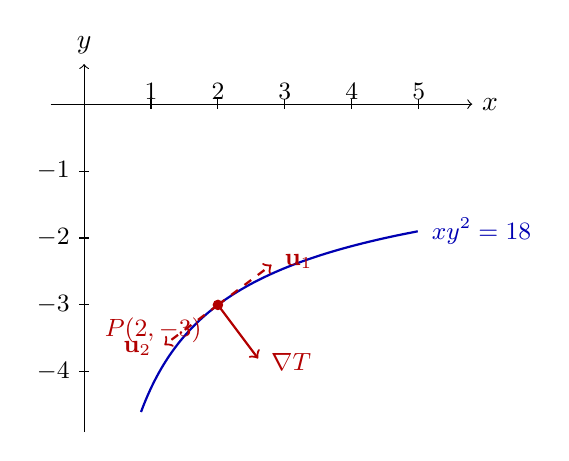
\begin{tikzpicture}[scale=0.85]
    % Ejes
    \draw[thin,->] (-0.5,0) -- (5.8,0) node[right] {$x$};
    \draw[thin,->] (0,-4.9) -- (0,0.6) node[above] {$y$};
    % Curva de nivel xy^2=18 (x=18/y^2), y in [-4.6,-1.9]
    \draw[thick, blue!70!black, variable=\t, domain=-4.6:-1.9, samples=50, smooth]
        plot ({18/(\t*\t)},{\t});
    \node[anchor=west, blue!70!black] at (5.05,-1.9)
        {\small $xy^2=18$};
    % Punto P(2,-3)
    \filldraw[red!70!black] (2,-3) circle (2pt);
    \node[anchor=north east, red!70!black] at (1.9,-3.05) {\small $P(2,-3)$};
    % Gradiente: direccion (3,-4)/5, escala 1.0
    \draw[->, thick, red!70!black] (2,-3) -- (2.6,-3.8);
    \node[anchor=west, red!70!black] at (2.65,-3.85) {\small $\nabla T$};
    % Direcciones con D_u T = 0: +-(4,3)/5, escala 1.0
    \draw[->, thick, red!70!black, dashed] (2,-3) -- (2.8,-2.4);
    \node[anchor=west, red!70!black] at (2.85,-2.35) {\small $\mathbf{u}_1$};
    \draw[->, thick, red!70!black, dashed] (2,-3) -- (1.2,-3.6);
    \node[anchor=east, red!70!black] at (1.15,-3.65) {\small $\mathbf{u}_2$};
    % Marcas de eje
    \foreach \xv in {1,2,3,4,5}
        \draw[thin] (\xv,0.07)--(\xv,-0.07) node[above] {\small $\xv$};
    \foreach \yv in {-1,-2,-3,-4}
        \draw[thin] (0.07,\yv)--(-0.07,\yv) node[left] {\small $\yv$};
\end{tikzpicture}
\caption{Direcciones $\mathbf{u}_1$, $\mathbf{u}_2$ con derivada direccional nula en $P(2,-3)$: son tangentes a la curva de nivel $xy^2=18$ (azul) y perpendiculares a $\nabla T(P)$}
\label{fig:du_nula_curva_nivel}
\end{figure}

\begin{prob}[Reconstrucción del gradiente a partir de derivadas direccionales]
En un punto $P$ se sabe que la derivada direccional de $f$ vale $2\sqrt2$ en
la dirección $\mathbf{u}=\tfrac1{\sqrt2}\langle 1,1\rangle$ y $\sqrt2$ en la
dirección $\mathbf{v}=\tfrac1{\sqrt2}\langle 1,-1\rangle$.
\begin{enumerate}[a)]
  \item Determine $\nabla f(P)$.
  \item ¿Existe alguna dirección $\mathbf{w}$ con $D_{\mathbf{w}}f(P)=4$?
\end{enumerate}
\begin{myproof}
\textbf{Paso 1. Plantear el sistema.}
Sea $\nabla f(P)=\langle a,b\rangle$. Como $D_{\mathbf u}f=\nabla f\cdot\mathbf u$,
\[
  \frac{a+b}{\sqrt2}=2\sqrt2,\qquad \frac{a-b}{\sqrt2}=\sqrt2,
\]
es decir $a+b=4$ y $a-b=2$.

\textbf{Paso 2. Resolver (a).}
Sumando y restando, $a=3$ y $b=1$:
\[
  \nabla f(P)=\langle 3,1\rangle,\qquad \|\nabla f(P)\|=\sqrt{10}.
\]

\textbf{Paso 3. Cota para (b).}
Para toda dirección unitaria $\mathbf w$,
$|D_{\mathbf w}f(P)|=|\nabla f\cdot\mathbf w|\le\|\nabla f(P)\|=\sqrt{10}\approx 3.16$.

\textbf{Paso 4. Conclusión.}
Como $4>\sqrt{10}$, \emph{no existe} tal dirección:
\[
  \boxed{\ \nabla f(P)=\langle 3,1\rangle;\quad
  \text{no hay }\mathbf w\text{ con }D_{\mathbf w}f(P)=4,\ \text{pues }
  |D_{\mathbf w}f|\le\sqrt{10}.\ }
\]
\end{myproof}
\end{prob}

%%----------------------------------------------------------
\section{Relación del plano tangente y la recta normal con el gradiente}
%%----------------------------------------------------------

En la sección anterior se introdujo el plano tangente a una superficie
determinada por una función explícita $z=f(x,y)$. Ahora se extiende este
concepto a superficies dadas en forma implícita $F(x,y,z)=k$. La
observación clave es que el gradiente $\nabla F$ es normal a la
superficie en cada punto.

\begin{rem}
Si la superficie está dada por $z=f(x,y)$, se puede expresar en forma
implícita como $F(x,y,z) = f(x,y) - z = 0$. Entonces
$\nabla F = \langle f_x, f_y, -1 \rangle$, que es un vector normal al
plano tangente. La ecuación
\[
f_x(x_0,y_0)(x-x_0) + f_y(x_0,y_0)(y-y_0) - (z-z_0) = 0
\]
recupera la fórmula del plano tangente para funciones explícitas
estudiada en la lección anterior.
\end{rem}

\begin{definition}[Plano tangente y recta normal para superficie implícita]
Sea $F(x,y,z)=k$ una superficie y supóngase que $F$ es diferenciable en
el punto $P(x_0,y_0,z_0)$, con $\nabla F(x_0,y_0,z_0) \neq \mathbf{0}$.
El \textbf{plano tangente} a la superficie en $P$ es el plano que pasa
por $P$ y es perpendicular a $\nabla F(P)$. La \textbf{recta normal} a
la superficie en $P$ es la recta que pasa por $P$ y tiene como vector
director $\nabla F(P)$.
\end{definition}

La ecuación del plano tangente en $(x_0,y_0,z_0)$ es:
\[
\nabla F(x_0,y_0,z_0) \cdot \langle x-x_0,\, y-y_0,\, z-z_0 \rangle = 0.
\]
Equivalentemente:
\[
F_x(x_0,y_0,z_0)(x-x_0)
+ F_y(x_0,y_0,z_0)(y-y_0)
+ F_z(x_0,y_0,z_0)(z-z_0) = 0.
\]

Las ecuaciones paramétricas de la recta normal son:
\[
x = x_0 + t\,F_x(x_0,y_0,z_0),\quad
y = y_0 + t\,F_y(x_0,y_0,z_0),\quad
z = z_0 + t\,F_z(x_0,y_0,z_0),\quad t\in\mathbb{R}.
\]

\begin{pasos}[Plano tangente a superficie implícita]
Para hallar el plano tangente y la recta normal a la superficie
$F(x,y,z)=k$ en el punto $P(x_0,y_0,z_0)$:
\begin{enumerate}
    \item \textbf{Función implícita.} Escribir la superficie en la forma
    $F(x,y,z)=k$ (si es necesario, restando $k$ de ambos lados).
    \item \textbf{Gradiente.} Calcular $\nabla F(x,y,z)$.
    \item \textbf{Evaluación.} Evaluar $\nabla F$ en $P$.
    \item \textbf{Ecuaciones.} Escribir la ecuación del plano usando
    $\nabla F(P)$ como vector normal, y las ecuaciones paramétricas de la
    recta usando $\nabla F(P)$ como vector director.
\end{enumerate}
\end{pasos}

\begin{example}[Plano tangente y recta normal a superficie implícita]
Halle las ecuaciones del plano tangente y la recta normal a la superficie
$x e^{yz} = 1$ en el punto $(1,0,5)$.
\begin{myproof}
Se sigue el protocolo para el plano tangente a superficie implícita.

\textbf{Paso 1. Función implícita.} Se define
\[
F(x,y,z) = x e^{yz} - 1 = 0.
\]
La superficie es $F(x,y,z)=0$.

\textbf{Paso 2. Gradiente.}
\[
\nabla F(x,y,z)
= \langle F_x, F_y, F_z \rangle
= \langle e^{yz},\, xz e^{yz},\, xy e^{yz} \rangle.
\]

\textbf{Paso 3. Evaluación en $P(1,0,5)$.}
\[
\nabla F(1,0,5)
= \langle e^{0\cdot 5},\, 1\cdot 5\cdot e^{0\cdot 5},\,
  1\cdot 0\cdot e^{0\cdot 5} \rangle
= \langle 1,\, 5,\, 0 \rangle.
\]

\textbf{Paso 4. Ecuaciones.}
El plano tangente tiene vector normal $\mathbf{n} = \langle 1,5,0 \rangle$
y pasa por $(1,0,5)$:
\[
1(x-1) + 5(y-0) + 0(z-5) = 0
\implies x - 1 + 5y = 0
\implies x + 5y = 1.
\]
La recta normal tiene vector director $\mathbf{v} = \langle 1,5,0 \rangle$
y pasa por $(1,0,5)$:
\[
x = 1 + t,\qquad y = 5t,\qquad z = 5,\qquad t\in\mathbb{R}.
\]
Por tanto:
\[
\boxed{\text{Plano tangente: } x + 5y = 1,\qquad
\text{Recta normal: } (x,y,z) = (1,0,5) + t\langle 1,5,0 \rangle}.
\]
\end{myproof}
\end{example}

\begin{prob}
Encuentre la ecuación del plano tangente y la recta normal a la
superficie en el punto indicado:
\begin{enumerate}[a)]
    \item $x^2 + y^2 + z^2 = 14$, $(1,2,3)$
    \item $x^2 + 2y^2 - z^2 = 4$, $(2,1,-1)$
    \item $xy + yz + zx = 1$, $(1,0,1)$
\end{enumerate}
\begin{myproof}
\textbf{Paso 1. Estrategia.}
Para $F(x,y,z)=c$: plano tangente $\nabla F(p)\cdot\langle x-x_0,y-y_0,z-z_0\rangle=0$; recta normal $\mathbf{r}(t)=p+t\,\nabla F(p)$.

\textbf{Paso 2 (a).} $F=x^2+y^2+z^2-14$, $p=(1,2,3)$.
\[
\nabla F=\langle 2x,2y,2z\rangle\big|_{(1,2,3)}=\langle 2,4,6\rangle.
\]
Plano: $2(x-1)+4(y-2)+6(z-3)=0\;\Rightarrow\;\boxed{x+2y+3z=14}$.
Recta: $\dfrac{x-1}{1}=\dfrac{y-2}{2}=\dfrac{z-3}{3}$.

\textbf{Paso 3 (b).} $F=x^2+2y^2-z^2-4$, $p=(2,1,-1)$.
\[
\nabla F=\langle 2x,4y,-2z\rangle\big|_{(2,1,-1)}=\langle 4,4,2\rangle.
\]
Plano: $4(x-2)+4(y-1)+2(z+1)=0\;\Rightarrow\;\boxed{2x+2y+z=5}$.
Recta: $\dfrac{x-2}{2}=\dfrac{y-1}{2}=\dfrac{z+1}{1}$.

\textbf{Paso 4 (c).} $F=xy+yz+zx-1$, $p=(1,0,1)$.
\[
\nabla F=\langle y+z,\,x+z,\,y+x\rangle\big|_{(1,0,1)}=\langle 1,2,1\rangle.
\]
Plano: $(x-1)+2y+(z-1)=0\;\Rightarrow\;\boxed{x+2y+z=2}$.
Recta: $\dfrac{x-1}{1}=\dfrac{y}{2}=\dfrac{z-1}{1}$.
\end{myproof}
\end{prob}

\begin{prob}[Rectas normales y superficies ortogonales]
\begin{enumerate}[a)]
  \item Demuestre que toda recta normal a la esfera $x^2+y^2+z^2=R^2$ pasa por
        el origen.
  \item Demuestre que la esfera $x^2+y^2+z^2=R^2$ y el cono $x^2+y^2=z^2$ se
        cortan ortogonalmente (sus normales son perpendiculares en cada punto
        de la intersección).
\end{enumerate}
\begin{myproof}
\textbf{Paso 1 (a). Recta normal a la esfera.}
Con $F=x^2+y^2+z^2-R^2$ se tiene $\nabla F=2\langle x,y,z\rangle$, así que en
$P=(x_0,y_0,z_0)$ la recta normal es
\[
  \mathbf{L}(t)=P+t\,\nabla F(P)=(1+2t)\,\langle x_0,y_0,z_0\rangle.
\]
Para $t=-\tfrac12$ resulta $\mathbf L(-\tfrac12)=\mathbf 0$: la recta pasa por
el origen. $\checkmark$

\textbf{Paso 2 (b). Gradientes de las dos superficies.}
Sea $F=x^2+y^2+z^2-R^2$ y $G=x^2+y^2-z^2$. Entonces
\[
  \nabla F=2\langle x,y,z\rangle,\qquad \nabla G=2\langle x,y,-z\rangle.
\]

\textbf{Paso 3. Producto escalar sobre la intersección.}
\[
  \nabla F\cdot\nabla G=4\,(x^2+y^2-z^2).
\]
En los puntos de intersección se cumple la ecuación del cono $x^2+y^2=z^2$,
luego $x^2+y^2-z^2=0$.

\textbf{Paso 4. Conclusión.}
\[
  \boxed{\ \nabla F\cdot\nabla G=0\ \text{sobre la intersección: las
  superficies son ortogonales.}\ }
\]
\end{myproof}
\end{prob}


%%==========================================================

\section{Problemas propuestos}
%%==========================================================
% Básico
\begin{prob}
Use la regla de la cadena para hallar $dz/dt$ si $z = \cos(x + 2y)$, $x = t^2$ e $y = \sen t$.
\end{prob}

\begin{prob}
El voltaje en los extremos de un conductor aumenta a una tasa de $9\ \text{V/min}$ y la resistencia disminuye a razón de $0{,}5\ \Omega/\text{min}$. Si $I=V/R$, calcule la tasa a la que cambia la corriente $I$ cuando $R=70\ \Omega$ y $V=60\ \text{V}$.
\end{prob}

\begin{prob}
Sean $f(x,y)=x^2-y^2$ y $g(x,y)=2xy$. Calcule el ángulo entre $\nabla f$ y
$\nabla g$ en el punto $(2,1)$ e interprete el resultado en términos de las
curvas de nivel de $f$ y $g$.
\end{prob}

\begin{prob}[Desafiante]
Halle constantes $a,b$ tales que la derivada direccional máxima de
$f(x,y)=e^{ax+by}\cos(x+y)$ en el origen valga $2\sqrt2$ y ocurra en la
dirección de la bisectriz del primer cuadrante.
\end{prob}

\begin{prob}[Gradiente y derivada direccional]
Calcule el gradiente de las siguientes funciones:
\begin{multicols}{2}
\begin{enumerate}
    \item $f(x,y) = x^2 y + \sen(xy)$
    \item $f(x,y) = \ln(x^2 + y^2)$
    \item $f(x,y,z) = xyz + e^{xz}$
    \item $f(x,y,z) = \arctan(x/y) + z^2$
\end{enumerate}
\end{multicols}
\end{prob}

\begin{prob}[Derivada direccional en tres variables]
Sea $f(x,y,z)=xy^2z^3$. Calcule la derivada direccional de $f$ en el punto
$P=(2,1,1)$ en la dirección del vector $\mathbf v=\langle 2,1,-2\rangle$.
(Sugerencia: $\nabla f=\langle y^2z^3,\ 2xyz^3,\ 3xy^2z^2\rangle$; normalice
$\mathbf v$ antes del producto escalar.)
\end{prob}


% Intermedio
\begin{prob}
La longitud $l$, ancho $a$ y altura $h$ de una caja cambia con el tiempo. En un cierto instante, las dimensiones son $l= 15\ m,$ $a=12\ m$ y $h= 3\ m$, y se conoce que $a$ y $h$ se incrementan a razón de $0.2\ m/s$, en tanto que $l$ disminuye a razón de $0.1\ m/s.$ Encuentre en ese instante las razones a las cuales el volumen de la caja cambia.
\end{prob}

\begin{prob}
La longitud $x,$ el ancho $y$ y la altura $z$ de una caja cambian con el tiempo. En cierto instante las dimensiones de la caja son $x=A\ cm,$ $y=2A\ cm$ y $z= 2A\ cm.$ Si $x$ y $y$ aumentan a una tasa de $2A\ cm/s$ mientras que $z$ disminuye a razón de $3A\ cm/s,$ emplee la regla de la cadena para determinar la tasa a la cual cambia el volumen de la caja en ese instante.
\end{prob}

\begin{prob}
La temperatura de una colina en un punto $(x,y,z)$ está dada por la función $$T(x,y,z)=200e^{-x^2-3y^2-9z^2}$$ donde $T$ se mide en grados Celsius y $x,\ y, \ z$ en metros.  Determine la dirección que un insecto seguiría, empezando en el punto $(2A,-A,2A)$ con el fin de calentarse lo más rápido posible. Justifique su respuesta.
\end{prob}

\begin{prob}
La longitud $x,$ el ancho $y$ y la altura $z$ de una caja cambian con el tiempo. En cierto instante las dimensiones de la caja son $x=7A\ cm,$ $y=13A\ cm$ y $z= 11A\ cm.$ Si $x$ y $y$ aumentan a una tasa de $2A\ cm/s$ mientras que $z$ disminuye a razón de $5A\ cm/s,$ emplee la regla de la cadena para determinar la tasa a la cual cambia el área superficial de la caja en ese instante (asuma que la caja tiene tapa).
\end{prob}


\begin{prob}
La temperatura de una colina en un punto $(x,y,z)$ está dada por la función $$T(x,y,z)=236e^{-13x^2-11y^2-17z^2}$$ donde $T$ se mide en grados Celsius y $x,\ y, \ z$ en metros.  Determine la dirección que un insecto seguiría, empezando en el punto $(3A,-7A,11A)$ con el fin de calentarse lo más rápido posible. Justifique su respuesta.
\end{prob}


\begin{prob}
Si $h(x,y)=2e^{-x^2}+3e^{-3y^2}$ representa la altura de una montaña, ¿en qué dirección desde $(1,0,2e^{-1}+3)$ se debería comenzar a caminar para escalar más rápidamente?
\end{prob}

\begin{prob}
La temperatura de una colina en un punto $(x,y,z)$ está dada por la función $$T(x,y,z)=258e^{-2x^2-5y^2-7z^2}$$ donde $T$ se mide en grados Celsius y $x,\ y, \ z$ en metros.  Determine la dirección que un insecto seguiría, empezando en el punto $(9A,-5A,13A)$ con el fin de calentarse lo más rápido posible. Justifique su respuesta.
\end{prob}

\begin{prob}
Considere una placa rectangular comprendida por el plano $xy$ cuya temperatura está determinada por  la función $T(x,y,z)=10+8x^2+25y^2$ donde $T$ se mide en grados Celsius y $x,\ y$ en metros.  Determine la dirección que un insecto seguiría, empezando en el punto $(A+1,A)$ con el fin de enfriarse lo más rápido posible. Justifique su respuesta.
\end{prob}


% Desafiante
\begin{prob}
La temperatura de una placa en un punto $(x,y)$ está dada por la función $$T(x,y)=10+5x^2-3y^2$$ donde $T$ se mide en grados Celsius y $x,\ y$ en metros.  Determine la dirección que un insecto seguiría, empezando en el punto $(3,-7)$ con el fin de calentarse lo más rápido posible. Justifique su respuesta.
\end{prob}

\begin{prob}
La temperatura de una placa en un punto $(x,y)$ está dada por la función $$T(x,y)=40+8x^2-25y^2$$ donde $T$ se mide en grados Celsius y $x,\ y$ en metros.  Determine la dirección que un insecto seguiría, empezando en el punto $(9,25)$ con el fin de calentarse lo más rápido posible. Justifique su respuesta.
\end{prob}

\begin{prob}
Considere una placa rectangular comprendida por el plano $xy$ cuya temperatura está dada por $T(x,y)=5+x^{2}+5y^{2}$ para cada punto $(x,y).$ Determine la dirección que un insecto seguiría, empezando en el punto $(A,A+1)$ con el fin de enfriarse lo más rápido posible. Justifique su respuesta.
\end{prob}

% [F9T.01 | propuesto | origen: T5.18, T5.19 | 3 incisos con direccion sin cambio]
\begin{prob}
Durante una reacción química sobre una placa, la temperatura en cada punto es $T(x,y)=-2x^3+6x^2y-5y^2.$ Un sensor se encuentra en el punto $(1,1).$
\begin{enumerate}[a)]
    \item ¿En qué dirección debe desplazarse el sensor para que la temperatura aumente lo más rápido posible, y cuál es esa tasa máxima de cambio?
    \item Calcule la derivada direccional de $T$ en $(1,1)$ en la dirección del vector $\mathbf{v}=\langle 3,-4\rangle.$
    \item Halle todas las direcciones en las que la temperatura no cambia instantáneamente y explique su relación con la curva de nivel de $T$ que pasa por $(1,1).$
\end{enumerate}
\end{prob}

\begin{prob}
La longitud del lado marcado $x$ del triángulo de la figura (no está construído a escala) aumenta a una tasa de $0.5\ cm/s$, el lado marcado $y$ crece a una tasa de $0.3\ cm/s$ y el ángulo $\theta$ aumenta a una tasa de $0.2\ rad/s.$ Emplee la regla de la cadena para determinar la tasa a la cual el área del triángulo está cambiando en el instante $x=13\ cm,$ $y=8\ cm$ y $\theta= \dfrac{\pi}{4}.$
\textit{Sugerencia: Determine cuál es la altura del triángulo en términos de $\theta$ tomando como base a $y.$}
\begin{figure}[H]
\centering
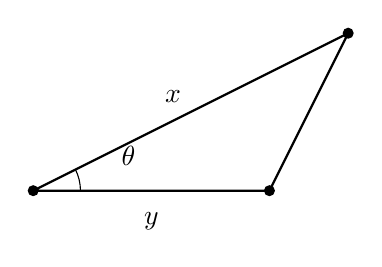
\begin{tikzpicture}[scale=1.0]
  \coordinate (O) at (0,0);
  \coordinate (A) at (3,0);
  \coordinate (B) at (4,2);
  \draw[thick] (O) -- (A) -- (B) -- cycle;
  \draw (0.6,0) arc[start angle=0, end angle=26.57, radius=0.6];
  \node[below] at (1.5,-0.15) {$y$};
  \node[above left] at (2,1) {$x$};
  \node[anchor=south west] at (1.0,0.2) {$\theta$};
  \fill (O) circle (2pt);
  \fill (A) circle (2pt);
  \fill (B) circle (2pt);
\end{tikzpicture}
\caption{Triángulo con lados $x$, $y$ y ángulo $\theta$ para el problema de razón de cambio.}
\label{fig:triangulo_cadena}
\end{figure}
\end{prob}
